% definiert einen neuen Counter für die Anforderungen
\newcounter{requirement} 
% Definiert ein neues Command für die Ausgabe der Anforderungen 
% Req Anforderungsnummer_aus_Counter: Text der Anforderung
\newcommand{\requirement}[1]{%
\refstepcounter{requirement}
\emph{Req~\arabic{requirement}:~#1}} 

%% setzt autoref in eine \emph Umgebung
\newcommand{\reqref}[1]{%
\emph{\autoref{#1}}} 

% Präfix Req für alle Anforderungsreferenzen
\def\requirementautorefname{Req}

\newcommand{\requirementRegistrieren}{Der Anwender muss sich selbständig in dem System registrieren können.} 
\newcommand{\requirementLogin}{Der Anwender muss sich sich in das System mit Nutzername und Passwort einloggen können.}
\newcommand{\requirementZugriffAufEigeneWidgets}{Dem Anwender darf nur Zugriff auf die zu seinem Account gehörigen Workspaces und Widgets gewährt werden.} 
\newcommand{\requirementLogout}{Der Anwender muss sich aus dem System ausloggen können.}
\newcommand{\requirementKeinZugriffNachLogout}{Nach Beendigung der Anwender-Session, darf kein Zugriff mehr auf die Daten des Anwenders bestehen.}
\newcommand{\requirementWorkspaceAdd}{Der Anwender muss neue Workspaces in seine Lernumgebung einfügen können.}
\newcommand{\requirementWorkspaceEdit}{Der Anwender muss den Namen des Workspaces ändern können.}
\newcommand{\requirementWorkspaceDelete}{Der Anwender muss einen Workspace löschen können.}
\newcommand{\requirementWidgetAdd}{Der Anwender muss über ein Auswahlfeld Widgets zu Workspaces hinzufügen können.}
\newcommand{\requirementWidgetFilterName}{Der Anwender muss die zur Auswahl stehenden Widgets über ein Suchfeld einschränken können.}
\newcommand{\requirementWidgetFilterOnline}{Der Anwender muss die zur Auswahl stehenden Widgets so einschränken können, dass in der Liste nur offline-fähige Widgets vorkommen.}
\newcommand{\requirementWidgetDelete}{Der Anwender muss ein Widget löschen können.}
\newcommand{\requirementWidgetSortDragNDrop}{Der Anwender muss in der Lage sein Widgets nach seinen Wünschen über einen Drag and Drop Mechanismus auf dem Workspace zu sortieren.}
\newcommand{\requirementWidgetInformSystem}{Die Widgets müssen dem System Informationen mitteilen können, welche Aufschluss über ihren Zustand geben. Diese sollen dem Nutzer dargestellt werden können.}
\newcommand{\requirementDashboard}{Das System muss dem Anwender eine Übersichtsseite über die verwendeten Workspaces und Widgets und ihre wichtigsten Informationen zur Verfügung stellen.}
\newcommand{\requirementCheckOnlineStatus}{Das System muss seinen Onlinestatus kennen, bemerken, wenn sich dieser ändert und dies dem Anwender mitteilen.}
\newcommand{\requirementOfflineStart}{Das System muss für die Applikation notwendigen Ressourcen zwischenspeichern, so dass es auch offline gestartet werden kann.}
\newcommand{\requirementOfflineWork}{Das System muss den Anwender in die Lage versetzen mit den gewählten Services, zumindest rudimentär, offline zu arbeiten.}
\newcommand{\requirementOnlineSync}{Bei einer Verbindung mit dem Internet müssen die offline vorgenommenen Arbeiten mit den Services synchronisiert werden.}
\newcommand{\requirementAggregator}{Das System muss als Aggregator für unterschiedliche externe Kanäle und Services dienen und dem Anwender die Arbeit mit ihnen an zentraler Stelle ermöglichen.}
\newcommand{\requirementWidgetStandard}{Die Services müssen über einen frei verfügbaren Standard in das System eingebunden werden können.}
\newcommand{\requirementUsbStick}{Die durchgeführten Arbeiten müssen offline zwischen unterschiedlichen Rechnern transportiert werden können.}
\newcommand{\requirementUsageInBrowser}{Das System muss in aktuellen Browsern mit nativen Browsertechnologien ohne weitere Installation nutzbar sein.}
\newcommand{\requirementExtensibility}{Das System muss einfach erweitert werden können.}
\newcommand{\requirementNewWidgetsWithApi}{Es muss möglich sein über eine API oder eine vorgegebene Implementierung neue Services und Kanäle mit Offlinefähigkeiten in das System zu laden.}
\newcommand{\requirementOpenSource}{Es dürfen keine proprietären, sondern nur freie Technologien für die Umsetzung des Systems genutzt werden.}

\chapter{Anforderungsanalyse} 
\label{chapter:Kapitel3}
\lhead{Kapitel 3. \emph{Anforderungsanalyse}}  

Das Ziel der vorliegenden Arbeit ist die prototypische Implementierung einer leichtgewichtigen Personal Learning Environment mit Offlinefähigkeiten auf Basis aktueller Technologien. Das vorliegende Kapitel beginnt mit dem Aufbau eines möglichen Szenarios, in dem die zu entwickelnde PLE zum Einsatz kommt. Auf Basis dieses Szenarios werden im folgenden Abschnit \ref{section:anwendungsfaelle} Anwendungsfälle erstellt und beschrieben. Aus diesen Anwendungsfälle werden die funktionalen Anforderungen an das System abgeleitet. In Abschnitt \ref{section:nichtfunktionale_anforderunge} werden anschließend weitere nichtfunktionale Anforderungen definiert. Das Kapitel schließt mit einer tabellarischen Auflistung der funktionalen und nichtfunktionalen Anforderungen.

\section{Ausgangssituation/Szenario}
Das in diesem Abschnitt vorgestellte Szenario beschreibt exemplarisch die mögliche Arbeit mit einer Personal Learning Environment und soll als Basis für die Anforderungen des in dieser Arbeit zu entwickelnden Systems dienen.

\subsection{Akteure}
\begin{itemize}
 \item Dozent mit Sitz in Hagen
 \item Student 1 mit Sitz in Kamerun (Fernuni Hagen)
 \item Student 2 mit Sitz in Kamerun (Fernuni Hagen)
 \item Student 3 mit Sitz in Berlin (Fernuni Hagen)
 \item Student 4 mit Sitz in Osnabrück (Universität Osnabrück) 
\end{itemize}

\subsection{Ausgangssituation}\label{section:ausgangssituation}
Der Dozent betreut an der Fernuni Hagen unter anderem den Kurs "`E-Learning: A new approach"'. Ziel dieses Kurses ist es die Lerntheorie des Konnektivismus (siehe \ref{section:konnektivismus}) unter Einsatz aktueller Technologien und Medien wie beispielsweise sozialer Netze, in einem realen Umfeld zum Einsatz zu bringen.  Für diesen Kurs hat der Dozent mehrere Kanäle zur Kommunikation angelegt. Die Studenten sollen die Kanäle wählen, die ihren Arbeitsgewohnten am meisten entsprechen. Am Ende des Semesters soll es eine Auswertung geben, welche Kanäle am häufigsten genutzt und welche von den Studenten eher ignoriert wurden. Parallel dazu werden die Systeme der Fernuni zur Online Bearbeitung der Einsendeaufgaben genutzt. Die vom Dozenten angelegten Kommunikationskanäle sind:
\begin{itemize}
 \item ein Twitter Channel
 \item einen eigenen Google-Calender
 \item einen Chat
 \item ein System zur Hinterlegug von Todo-Listen
 \item einen eigenen Blog, welcher einen RSS Feed bereitstellt 
\end{itemize}
Die Studenten sind angehalten sich regelmäßig über Aktualisierungen der Kanäle auf dem Laufenden zu halten. Für diesen Kurs haben sich die Studenten 1 und 3 eingeschrieben.

Zusätzlich haben sich Student 1, 2 und 4 zu einer virtuellen Lerngruppe zum Thema Datenbanken zusammengeschlossen. Hierfür können nicht die Systeme der Fernuni Hagen genutzt werden, da nur Student 2 momentan in dem spezifischen Kurs eingeschrieben ist. Student 1 hat sich nicht für den Kurs angemeldet und Student 4 hat überhaupt keine Möglichkeit dazu, da er nicht an der Fernuni immatrikuliert ist. Sie haben sich dazu entschlossen primär einen Chat zur Kommunikation zu benutzen.

Student 1 und Student 2 leben in Kamerun. Beide haben dort das Problem, dass der Internetzugriff aus mehreren Gründen nicht immer gegeben ist. Student 1 hat zu Hause keinen Internetzugang. Er hat nur die Möglichkeit in der Universität oder in einem Internetcafe online zu gehen. Student 2 hat einen Internetzugang, allerdings ist dieser relativ langsam und wird nach Zeit abgerechnet, so dass es vorteilhaft für ihn ist, wenn er nur für kurze Zeit online ist. Aus diesem Grund benötigen die beiden idealerweise ein System, welches ihnen die Möglichkeit bietet die neuesten Informationen auch offline zu lesen und zumindest rudimentär auch offline kleine Aufgaben zu erledigen. Diese sollten sich bei Wiederverbindung mit dem Internet mit den entsprechenden Services synchronisieren. Des Weiteren sollten sie in der Lage sein die Daten auch ohne Internetverbindung zwischen verschiedenen Rechnern auszutauschen. Insbesondere Student 1 sollte in der Lage seine Aktionen bei sich zu Hause vorzunehmen und die durchgeführten Änderungen dann an einem Rechner mit Internetanschluss zu synchronisieren. Die Anforderungen von Student 3 sind ähnlich gelagert. Er ist sehr viel unterwegs und erledigt daher viele kurze Aufgaben mit dem Smartphone. Auch hier ist eine Internetverbindung nicht immer gewährleistet ist oder sie wird temporär deaktiviert um die Akkulaufzeit zu verlängern. Durch die Arbeit an unterschiedlichen Rechnern mit potentiell unterschiedlichen Betriebssystemen, ist die Installation einer komplexen Software nicht ohne Weiteres möglich.
Idealerweise nutzen alle Studenten das selbe Basissystem und können sich hier die benötigten Services und Applikationen so zusammenstellen wie es ihren Ansprüchen entspricht.

\subsection{Arbeitsabläufe}
Im Folgenden werden die unterschiedlichen Arbeitsabläufe mit dem System exemplarisch an Student 1 und an Student 3 dargelegt.

\subsubsection*{Grundsätzlicher Arbeitsablauf für Studenten}
Um mit der PLE arbeiten zu können müssen die Studenten als erstes online eine Account in dem PLE-System erstellen. Anschließend melden sie sich mit ihren gewählten Login-Daten an. Bei erfolgreicher Anmeldung hat der Anwender die Möglichkeit direkt Workspaces zu erstellen, mit diesen zu arbeiten (Workspace umbenennen, Einstellungen vornehmen, Widgets hinzufügen etc).

\subsubsection*{Arbeitsablauf Student 1}
\begin{itemize}
 \item \emph{Tag 1:} Student 1 befindet sich in der Universität und verbindet seinen USB-Stick mit einem PC. Auf diesem Stick befindet sich die ausführbare mobiler Version eines aktuellen Browsers. Er öffnet die Applikation online in diesem Browser (alle folgenden Aktionen werden mit dem selben Browser durchgeführt). Student 1 erstellt einen neuen Workspace und benennt ihn in "`PLE"' um. Anschließend sucht er die Widgets für den PLE Workspace aus der Widget-Datenbank heraus. Das System zeigt ihm dabei an, für welche Widgets eine Offline-Fähigkeit zur Verfügung steht. Daraufhin organisiert er die Anordnung der Widgets nach seinen Vorstellungen per Drag and Drop neu. Damit er mit den einzelnen Widgets auch arbeiten kann, meldet sich Student 1 schließlich bei den jeweiligen Services mit seinen Account-Daten an. Bevor er den Browser schließt haben sich alle Widgets mit ihren Services synchronisiert und zeigen ihm dies auch an.
 \item \emph{Tag 2:} Student 1 loggt sich an der Uni in das PLE-System ein. Das System zeigt ihm auf der Startseite (dem Dashboard) an wie viele neue Items es auf seinem PLE Workspace gibt. Ein direkter Link führt ihn zum Workspace. Er sieht, dass momentan mehrere Leute im Chat sind und unterhält sich über das Widget mit ihnen. Der Dozent hat einige globale Todos angelegt und die ersten Nachrichten kommen über den Twitter Channel herein. Er sieht, dass Student 3 einen längeren Text im Chat geschrieben hat, beschließt diesen jedoch später zu lesen. Gleiches gilt für den Einführungsartikel des Dozenten im Kursblog. Hierfür erstellt er sich Items in seiner Todo-Liste. Abschließend schließt Student 1 den Browser und entfernt den USB-Stick.
 \item \emph{Tag 3:} Student 1 öffnet die Applikation in seinem mobilen Browser zu Hause. Das System erkennt, dass es sich im Offline-Modus befindet und versucht keine Synchronisierung mit dem Internet herzustellen. Student 1 liest den Text, den Student 3 im Chat hinterlegt hat und beantwortet die darin gestellten Fragen ebenfalls im Chatfenster. Anschließend teilt er dies über Twitter mit und erledigt sein Todo-Item.
 \item \emph{Tag 4:} Student 1 loggt sich im Internet-Cafe mit seinem mobilen Browser in das System ein. Das System erkennt, dass es online ist, lädt die neuesten Items der Services herunter und synchronisiert die nur lokal vorgenommenen Aktionen (Twitter, Chat, Todo). Per Mail hat Student 1 den Vorschlag von Student 2 bekommen gemeinsam mit Student 4 eine Lerngruppe zum Thema Datenbanken zu gründen. Hierzu wollen sie unter anderem ein Chat-System benutzen. Student 1 schlägt per Mail das ihm bekannte Chat-Widget für die PLE-Applikation vor. Er erstellt einen neuen Workspace, nennt ihn “Lerngruppe DB” und fügt das Chat-Widget mit den passenden Einstellungen hinzu.
 \item \emph{Tag 5:} Student 1 sieht in seinem Dashboard, dass es für den Workspace “Lerngruppe DB” 12 neue Items gibt. Er geht direkt zu dem Workspace und stellt fest, dass die beiden anderen Studenten sich ebenfalls in dem Chat angemeldet haben. Da momentan alle online verfügbar sind, beginnen sie ihre erste Gruppenunterhaltung und planen die weitere Vorgehensweise.
\end{itemize}

\subsubsection*{Arbeitsablauf Student 3}
Student 3 nutzt das System hauptsächlich mit seinem Tablet, welches in der Lage ist sich über Wlan, sowie UMTS mit dem Internet zu verbinden.

\begin{itemize}
 \item \emph{Tag 1:} Student 3 meldet sich ähnlich wie Student 1 in der PLE an und erstellt für seine Uni-Kurse jeweils einen Workspace. Außerdem legt er sich einen Workspace an, in dem sich nicht kursspezifische Widgets finden. Hierzu gehören, sein RSS-Reader, eine Todo Liste, sowie ein Google-Calender-Widget
 \item \emph{Tag 2:} Student 3 verbindet sich zu Hause mit seinem Wlan und loggt sich in der PLE ein. Nach Prüfung des Dashboards erstellt er sich in der allgemeinen Todo Liste für den Tag. Er sieht, dass es in seinem RSS-Reader 9 neue Artikel gibt. Diese möchte er auf seinem Weg zur Uni in der U-Bahn lesen. Auf dem Weg in die Universität ruft Student 3 das System auf seinem Tablet auf. Da kein Internetzugang besteht greift das System nur auf die lokalen Daten zurück. Das Calender-Widget in seinem globalen Workspace ist nicht offline-fähig. Aus diesem Grund wird es auch nur ausgegraut und nicht-funktional angezeigt. Der Student ist jedoch in der Lage seine lokal gecachten RSS-Artikel zu lesen. Bei Lektüre eines Artikels über Javascript fällt ihm ein, dass er sein Uni-Projekt noch mit der neuesten JQuery Version updaten wollte. Hierzu erstellt er sich ein weiteres Todo auf seiner Liste.
 In der Uni verbindet er sein Tablet mit dem Uni-Wlan. Der RSS-Reader markiert die 6 Artikel die, Student 3 in der U-Bahn gelesen hat als gelesen und synchronisiert das neueste Todo-Item mit dem Service im Internet.  
\end{itemize}

Zusammenfassend kann also gesagt werden, dass Betreuer und Studenten stehen über unterschiedliche Kanäle in Kommunikation miteinander stehen. Es müssen Termine geplant oder auch Notizen und Nachrichten hin und hergeschickt werden. Diese Kanäle sollen auf einem zentralen Zugang so zusammengefasst sein, dass es den Teilnehmern des Kurse alle relevanten Informationen an einer aufrufen und bearbeiten zu können. Dabei sind die Teilnehmer zu unterschiedlichen Zeiten online. Die Teilnehmer sollen das System offline Nutzen können, um einfache Arbeiten wie das Schreiben von Twitter-Nachrichten, Notizen und Instant-Messaging Nachrichten oder eine Terminabsprache über einen Kalender erledigen können. Bei dem Wechsel zwischen Online und Offline müssen die Daten synchronisiert werden. Idealerweise haben die Nutzer alle Daten auf einem USB-Stick bei sich und können so von unterschiedlichsten Rechnern, wie beispielsweise in der Universität, im Internetcafe oder zu von Hause aus, arbeiten.

\section{Anwendungsfälle/Funktionale Anforderungen}\label{section:anwendungsfaelle}
\begin{figure}[hb]
  \centering
  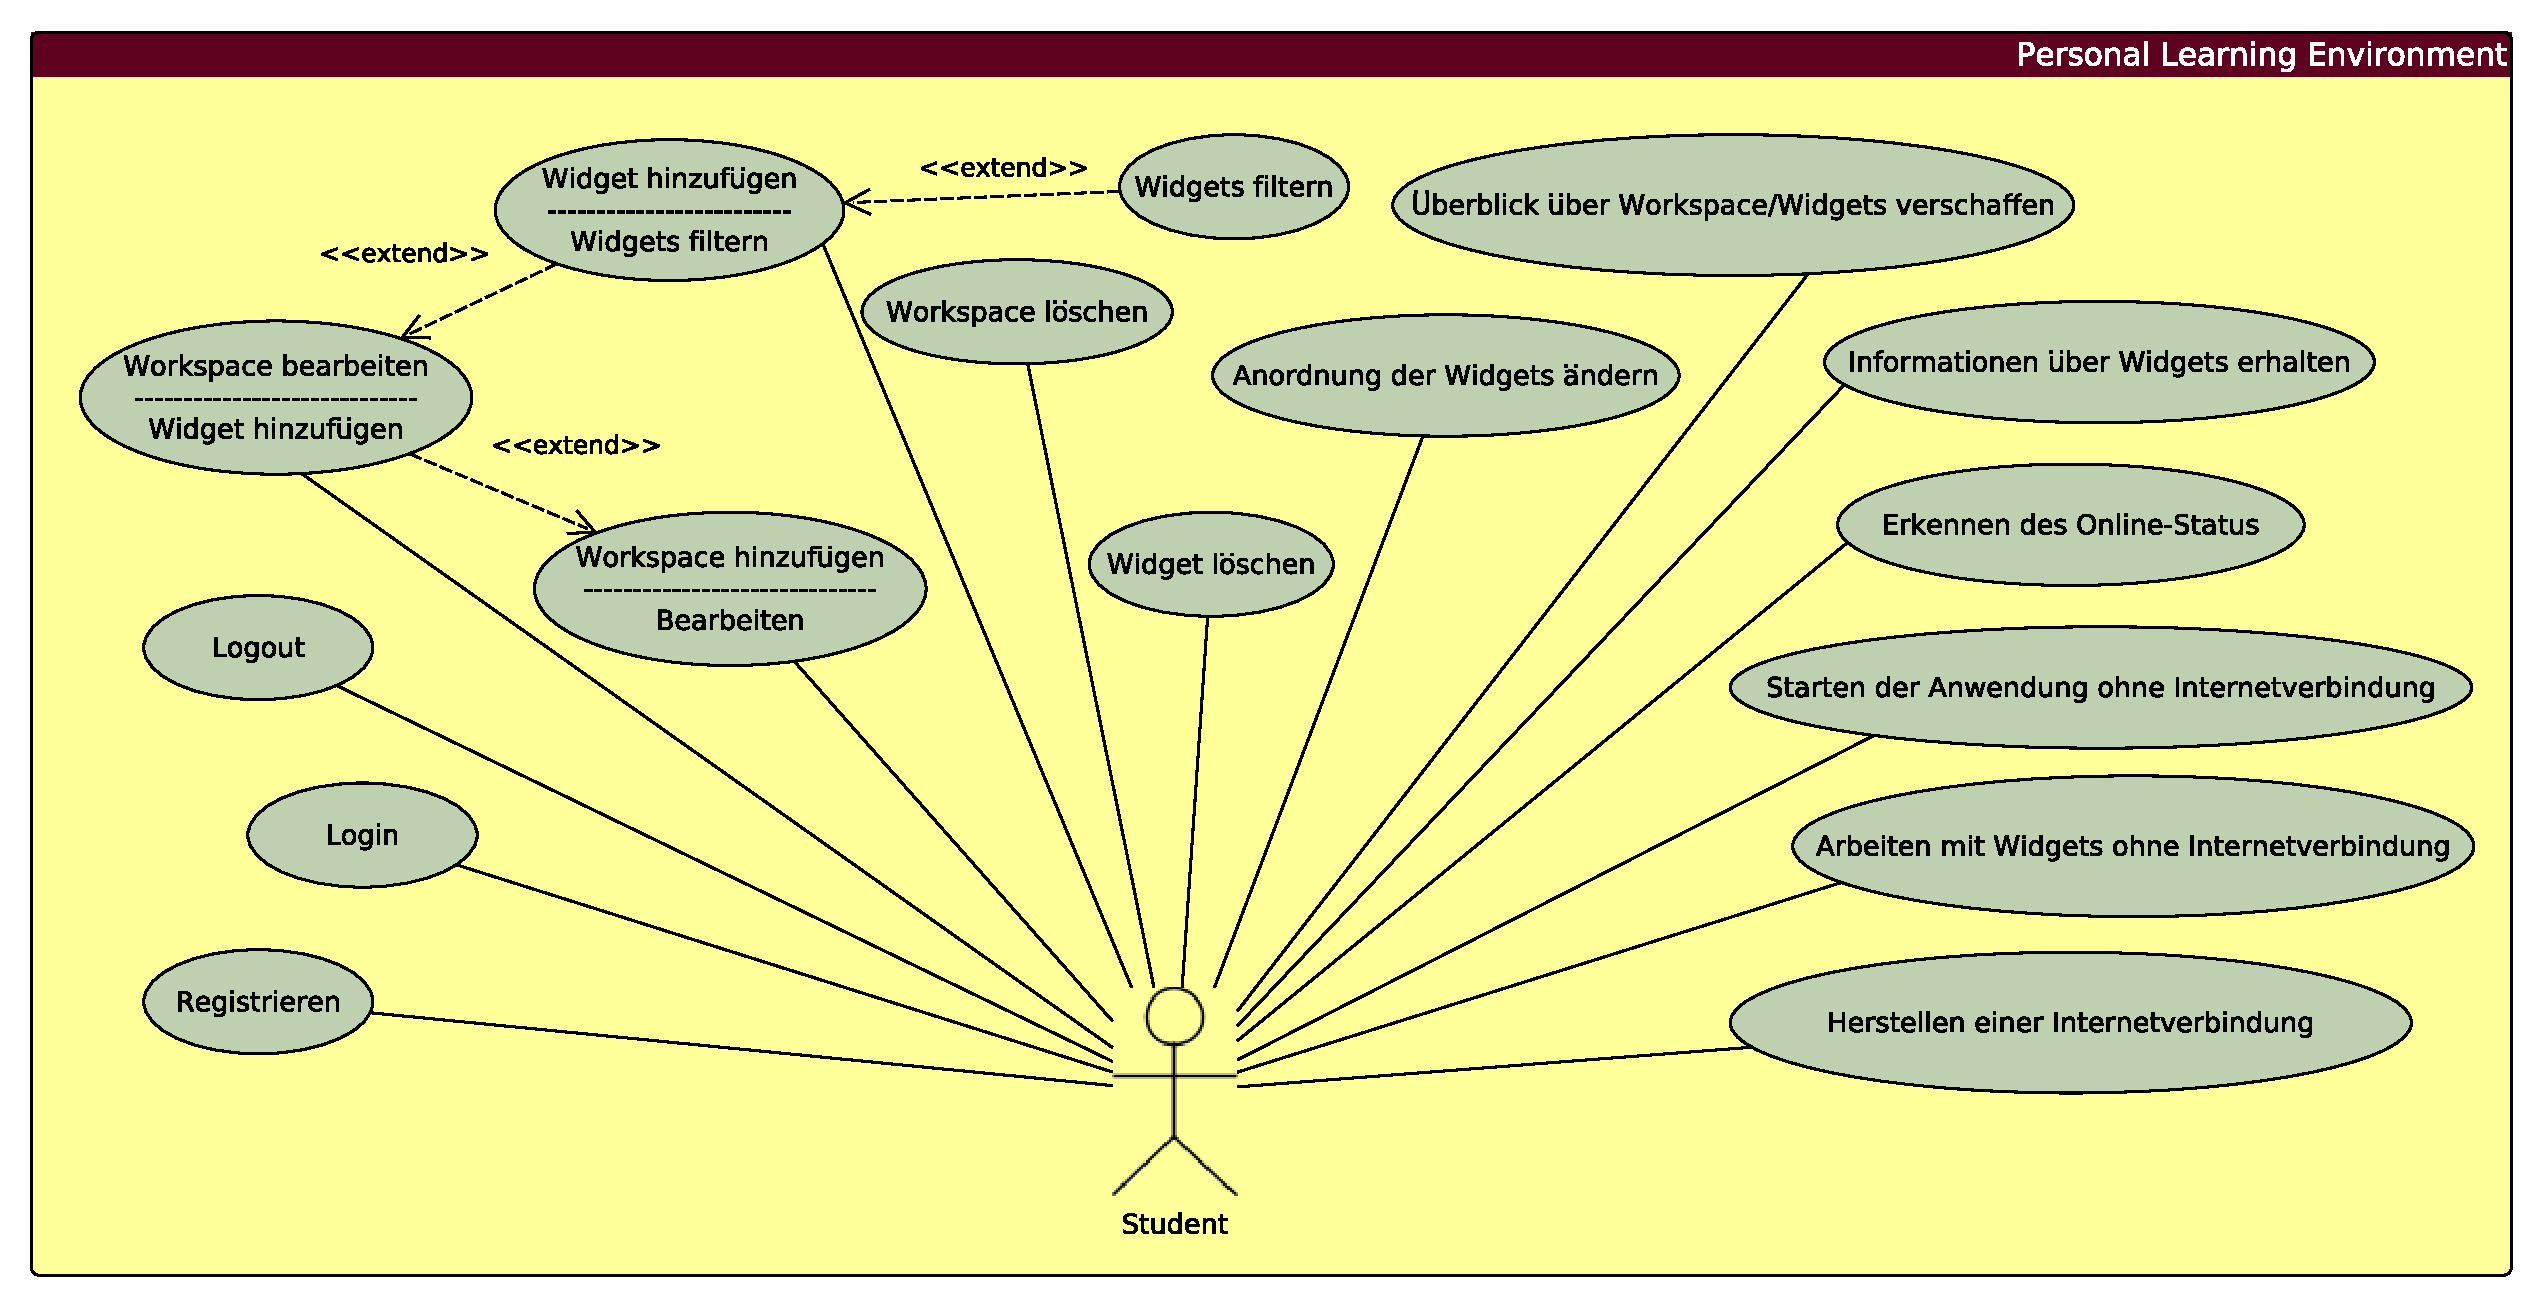
\includegraphics[width=\textwidth,height=\textheight,keepaspectratio]{./Figures/anwendungsfaelle_quer.pdf}
    \rule{35em}{0.5pt}
  \caption[Anwendungsfälle der PLE]{Die wichtigsten Anwendungsfälle für die PLE}
  \label{fig:anwendungsfaelle}
\end{figure}

Abbildung \ref{fig:anwendungsfaelle} zeigt die in dem eben aufgestellten Szenario auftretenden Anwendungsfälle. Diese werden im folgenden in textueller Form beschrieben. Aus diesen Beschreibungen werden dann direkt die funktionalen Anforderungen an das zu entwickelnde System abgeleitet.

\subsection{Registrieren}
\textbf{use case} \emph{Registrieren}\\
\textbf{actors} Student\\
\textbf{precondition} Das System ist online, der Student ist nicht eingeloggt und es existiert mindestens ein Workspace.\\
\textbf{main flow} Der Student bekommt auf der Startseite die Möglichkeit sich für den Zugang zum System zu registrieren. Er füllt ein Formular mit seinen Daten (Vorname, Nachname, E-Mailadresse, Nutzername, Passwort) aus und schickt das Formular ab.\\
\textbf{postcondition} Der Student ist mit einer Nutzername-/Passwortkombination und seiner E-Mailadresse im System hinterlegt und kann sich somit in das System einloggen.\\
\textbf{exceptional flow} Nutzername oder Mail-Adresse bereits vorhanden. Nutzername und E-Mail-Adresse dürfen nur einmal im System vorkommen.\\
\textbf{postcondition} Der Student bekommt eine Fehlermeldung und muss seine eingetragenen Daten ändern.
 
Aus diesem Anwendungsfall folgt die funktionale Anforderung \reqref{requirementRegistrieren}:\\
\requirement{\requirementRegistrieren}\label{requirementRegistrieren}\\
 
\subsection{Login}
\textbf{use case} \emph{Login}\\
\textbf{actors} Student\\
\textbf{precondition} Das System ist online, der Student ist nicht eingeloggt, ist aber in dem System registriert.\\
\textbf{main flow} Der Student bekommt auf der Startseite die Möglichkeit sich im System anzumelden. Er füllt ein Formular mit seiner Nutzername-/Passwortkombination aus und schickt das Formular ab.\\
\textbf{postcondition} Der Student ist im System eingeloggt und das System präsentiert ihm eine Übersicht über seine aktuellen Workspaces und die wichtigsten aggregierten Informationen dieser.
 
Aus diesem Anwendungsfall folgen die funktionalen Anforderungen \reqref{requirementLogin} und \reqref{requirementZugriffAufEigeneWidgets}:\\
\requirement{\requirementLogin}\label{requirementLogin}\\
\requirement{\requirementZugriffAufEigeneWidgets}\label{requirementZugriffAufEigeneWidgets}\\

 \subsection{Logout}
\textbf{use case} \emph{Logout}\\
\textbf{actors} Student\\
\textbf{precondition} Das System ist online, der Student ist eingeloggt.\\
\textbf{main flow} Der Student wählt die Aktion "`Logout"' und wird anschließend auf die Login-Seite weitergeleitet.\\
\textbf{postcondition} Die aktuelle Session des Anwenders ist beendet und es ist ohne weiteres Login nicht möglich auf die Daten des Anwenders zuzugreifen 
 
Aus diesem Anwendungsfall folgen die funktionale Anforderung \reqref{requirementLogout} und \reqref{requirementKeinZugriffNachLogout}:\\
\requirement{\requirementLogout}\label{requirementLogout}\\
\requirement{\requirementKeinZugriffNachLogout}\label{requirementKeinZugriffNachLogout}\\
 
\subsection{Workspace hinzufügen}
\textbf{use case} \emph{Workspace hinzufügen}\\
\textbf{actors} Student\\
\textbf{precondition} Das System ist online, der Student ist eingeloggt.\\
\textbf{main flow} Der Student wählt die Aktion "`Workspace hinzufügen"'. Es öffnet sich hierdurch ein neuer Bereich, welcher einen neuen Workspace repräsentiert. Der Student hat nun die Möglichkeit den Workspace nach seinen Wünschen anzupasssen (extension point: Workspace bearbeiten).\\
\textbf{postcondition} Ein neuer Workspace wurde dem System des Studenten hinzugefügt.
 
Aus diesem Anwendungsfall folgt die funktionale Anforderungung \reqref{requirementWorkspaceAdd}:\\
\requirement{\requirementWorkspaceAdd}\label{requirementWorkspaceAdd}\\
 
\subsection{Workspace bearbeiten}
\textbf{use case} \emph{Workspace bearbeiten}\\
\textbf{actors} Student\\
\textbf{precondition} Das System ist online, der Student ist eingeloggt und es existiert mindestens ein Workspace.\\
\textbf{main flow} Der Student wählt bei einem Workspace die Aktion "`Workspace bearbeiten"'. Der Anwender hat nun die Möglichkeit den Workspace nach seinen Wünschen zu benennen und kann Widgets zu dem Workspace hinzufügen (extension point: Widget hinzufügen).\\
\textbf{postcondition} Der Workspace wurde nach den Vorstellungen des Akteures angepasst.
 
\textbf{extend relationship}\\
\textbf{base} "`Workspace hinzufügen"'\\
\textbf{extensionPoint} Workspace bearbeiten\\
\textbf{extension} "`Workspace bearbeiten"'
 
Aus diesem Anwendungsfall folgt die funktionale Anforderungung \reqref{requirementWorkspaceEdit}:\\
\requirement{\requirementWorkspaceEdit}\label{requirementWorkspaceEdit}\\
 
\subsection{Workspace löschen}
\textbf{use case} \emph{Workspace löschen}\\
\textbf{actors} Student\\
\textbf{precondition} Das System ist online, der Student ist eingeloggt und es existiert mindestens ein Workspace.\\
\textbf{main flow} Der Student wählt bei einem Workspace die Aktion "`Workspace löschen"'. Es erscheint eine Rückfrage, welche eine Bestätigung des Löschvorganges (mitsamt aller Widgets) erfragt. Bei positiver Rückmeldung gibt das System die Nachricht des Löschens aus. \\
\textbf{postcondition} Der Workspace und alle seine Widgets sind aus dem System entfernt.
 
Aus diesem Anwendungsfall folgt die funktionale Anforderungung \reqref{requirementWorkspaceDelete}:\\
\requirement{\requirementWorkspaceDelete}\label{requirementWorkspaceDelete}\\

\subsection{Widget hinzufügen}
\textbf{use case} \emph{Widget hinzufügen}\\
\textbf{actors} Student\\
\textbf{precondition} Das System ist online, der Student ist eingeloggt und es existiert mindestens ein Workspace.\\
\textbf{main flow} Der Student befindet sich in einem Workspace und wählt die Aktion "`Widget hinzufügen"' Es erscheint eine Maske in der die zur Verfügung stehenden Widgets ausgewählt werden können. Der Student wählt das gewünschte Widget und fügt es dem Workspace hinzu. Wenn gewünscht kann der Student die Liste der Widgets über Suchfilter einschränken (extension point: Widgets filtern)\\
\textbf{postcondition} Das Widget wurde dem Workspace hinzugefügt.

\textbf{extend relationship}\\
\textbf{base} `Workspace bearbeiten"'\\
\textbf{extensionPoint} Widget hinzufügen\\
\textbf{extension} "`Widget hinzufügen"'

Aus diesem Anwendungsfall folgt die funktionale Anforderungung \reqref{requirementWidgetAdd}:\\
\requirement{\requirementWidgetAdd}\label{requirementWidgetAdd}\\

\subsection{Widgets Filtern}
\textbf{use case} \emph{Widgets Filtern}\\
\textbf{actors} Student\\
\textbf{precondition} Der Student ist dabei einem Workspace ein Widget hinzuzufügen.\\
\textbf{main flow} Der Student gibt in einem Textfeld eine Zeichenkette an, nach der im Widgetnamen gesucht wird. Des weiteren kann er in einem binären Filter wählen, ob er nur Widgets angezeigt bekommen möchte, die in der Lage sind in einem Offline-Modus zu arbeiten.\\
\textbf{postcondition} In der Liste der zur Auswahl stehenden Widgets werden nur noch diejenigen angezeigt, die der Filterung entsprechen.
 
\textbf{extend relationship}\\
\textbf{base} "`Widget hinzufügen"'\\
\textbf{extensionPoint} Widgets filtern\\
\textbf{extension} "`Widgets filtern"'
 
Aus diesem Anwendungsfall folgen die funktionalen Anforderungen \reqref{requirementWidgetFilterName} und \reqref{requirementWidgetFilterOnline}:\\
\requirement{\requirementWidgetFilterName}\label{requirementWidgetFilterName}\\
\requirement{\requirementWidgetFilterOnline}\label{requirementWidgetFilterOnline}\\
 
\subsection{Widget löschen}
\textbf{use case} \emph{Widget löschen}\\
\textbf{actors} Student\\
\textbf{precondition} Das System ist online, der Student ist eingeloggt, er und es existiert mindestens ein Widget auf einem Workspace.\\
\textbf{main flow} Der Student befindet sich in einem Workspace und wählt bei einem Widget die Aktion "`Widget löschen"'. Es erscheint eine Rückfrage, welche eine Bestätigung des Löschvorganges erfragt. Bei positiver Rückmeldung gibt das System die Nachricht des Löschens aus.
\textbf{postcondition} Das Widget wurde aus dem System entfernt.
 
Aus diesem Anwendungsfall folgt die funktionale Anforderungung \reqref{requirementWidgetDelete}:\\
\requirement{\requirementWidgetDelete}\label{requirementWidgetDelete}\\
 
\subsection{Anordnung der Widgets ändern}
\textbf{use case} \emph{Anordnung der Widgets ändern}\\
\textbf{actors}Student\\
\textbf{precondition} Das System ist online, der Student ist eingeloggt und befindet sich auf der Seite eines Workspaces mit mindestens zwei Widgets.\\
\textbf{main flow} Der Student hat die Möglichkeit die einzelnen Widgets innerhalb eines Workspaces über einen Drag and Drop Mechanismus neu anzuordnen. Er wählt hierfür ein Widget mit der Maus aus und zieht es an die gewünschte Position.\\
\textbf{postcondition} Die Anordnung der Widgets innerhalb des Workspaces hat sich nach dem Wunsch des Studenten geändert.
 
Aus diesem Anwendungsfall folgt die funktionale Anforderungung \reqref{requirementWidgetSortDragNDrop}:\\
\requirement{\requirementWidgetSortDragNDrop}\label{requirementWidgetSortDragNDrop}\\

\subsection{Informationen über Widgets erhalten}
\textbf{use case} \emph{Informationen über Widgets erhalten}\\
\textbf{actors}Student\\
\textbf{precondition} Der Student ist eingeloggt bewegt sich zu einem Workspace Workspace.\\
\textbf{main flow} Die Widgets des Workspaces aktualisieren sich mit ihren Services. \\
\textbf{postcondition} Jedes Widget zeigt ihm die wichtigsten Informationen an. Hierzu gehören, wie viele neue Items/Einträge (je nach Widget) es gibt, wie viele eventuell noch nicht mit dem Backend synchronisiert sind und ob das Widget online oder offline ist.
 
Aus diesem Anwendungsfall folgt die funktionale Anforderungung \reqref{requirementWidgetInformSystem}:\\
\requirement{\requirementWidgetInformSystem}\label{requirementWidgetInformSystem}\\

\subsection{Überblick über Workspace/Widgets verschaffen}
\textbf{use case} \emph{Überblick verschaffen}\\
\textbf{actors}Student\\
\textbf{precondition} Der Student ist eingeloggt.\\
\textbf{main flow} Der Student wählt eine Aktion aus, die in zu einer Übersichtsseite innerhalb des Systems bringt.\\
\textbf{postcondition} Der Student befindet sich auf einer Seite, welche ihm seine Workspaces und Widgets anzeigt und ihm die wichtigsten Informationen darüber vermittelt.

Aus diesem Anwendungsfall folgt die funktionale Anforderungung \reqref{requirementDashboard}:\\
\requirement{\requirementDashboard}\label{requirementDashboard}\\

\subsection{Erkennen des Onlinestatus}
\textbf{use case} \emph{Erkennen des Onlinestatus}\\
\textbf{actors}Student\\
\textbf{precondition} er Student ist eingeloggt, das System ist online\\
\textbf{main flow} Der Student sieht auf den ersten Blick, dass das System Online ist. Sowohl die Hauptapplikation, als auch die Widgets zeigen ihm dies an. Der Nutzer beendet die Interverbindung.\\
\textbf{postcondition} Das System zeigt dem Nutzer den Verlust der Verbindung direkt an.
 
Aus diesem Anwendungsfall folgt die funktionale Anforderungung \reqref{requirementCheckOnlineStatus}:\\
\requirement{\requirementCheckOnlineStatus}\label{requirementCheckOnlineStatus}\\

\subsection{Starten der Anwendung ohne Internetverbindung}
\textbf{use case} \emph{Starten der Anwendung ohne Internetverbindung}\\
\textbf{actors}Student\\
\textbf{precondition} Es besteht keine Internetverbindung.\\
\textbf{main flow} Der Anwender öffnet seinen Browser und gibt die URL der PLE ein.\\
\textbf{postcondition} Das System hat sich trotz fehlender Interverbindung geöffnet stellt dem Studenten das ihm bekannte User-Interface dar.
 
Aus diesem Anwendungsfall folgt die funktionale Anforderungung \reqref{requirementOfflineStart}:\\
\requirement{\requirementOfflineStart}\label{requirementOfflineStart}\\

\subsection{Arbeiten mit Widgets ohne Internetverbindung}
\textbf{use case} \emph{Arbeiten mit Widgets ohne Internetverbindung}\\
\textbf{actors}Student\\
\textbf{precondition} Das System ist geladen, hat aber keine Internetverbindung.\\
\textbf{main flow} Der Anwender arbeitet mit den Widgets und kann neue Einträge etc hinzufügen und bearbeiten.\\
\textbf{postcondition} Die Änderungen wurden zwischengespeichert. Dies wird dem Nutzer angezeigt.

Aus diesem Anwendungsfall folgt die funktionale Anforderungung \reqref{requirementOfflineWork}:\\
\requirement{\requirementOfflineWork}\label{requirementOfflineWork}\\

\subsection{Herstellen einer Internetverbindung}
\textbf{use case} \emph{Herstellen einer Internetverbindung}\\
\textbf{actors}Student\\
\textbf{precondition} Das System ist offline. Der Student hat in den Widgets Einträge hinzugefügt, bearbeiten oder gelöscht.\\
\textbf{main flow} Der Student stellt eine Verbindung mit dem Internet her.\\
\textbf{postcondition} Die offline vorgenommenen Arbeiten wurden mit dem jeweiligen Backend synchronisiert.

Aus diesem Anwendungsfall folgt die funktionale Anforderungung \reqref{requirementOnlineSync}:\\
\requirement{\requirementOnlineSync}\label{requirementOnlineSync}\\

\section{Nichtunktionale Anforderungen}\label{section:nichtfunktionale_anforderunge}

\subsection{Voraussetzungen}
Wie in Kapitel \ref{chapter:Kapitel2} beschrieben sind Personal Learning Environments Mashup-Anwendungen, welche unterschiedliche Anwendungen zu einem System zusammenfassen. Diese Anwendungen sind Services oder Kanäle, wie zum Beispiel Twitter, Facebook oder auch Applikationen für Todo-Listen oder Chats. Das System muss also als Aggregator fungieren, welcher diese Anwendungen in einer Anwendung bündelt und dem Nutzer in übersichtlicher Form präsentiert und ihm die Arbeit mit ihnen ermöglicht. Die in den funktionalen Anforderungen beschriebenen Widgets stellen hierbei die Umsetzung dieser Applikationen in der PLE dar. Diese Widgets sollten in der Lage sein wichtige Informationen an das System zu kommunizieren, so dass diese für den Nutzer aufbereitet und zusammengefasst dargestellt werden können. Dem Nutzer sollten genügend Services für seine PLE zur Verfügung stehen und die Entwicklung sollte nicht von einer Person oder Firma abhängen. Aus diesem Grund muss für die Einbindung der Services ein frei verfügbarer Standard und keine proprietäre Schnittstelle verwendet werden. Die Daten sollen auch ohne Internetverbindung zwischen verschiedenen Rechnern ausgetauscht werden können, so dass gewisse Arbeiten an einem Rechner durchgeführt werden können und diese Arbeiten dann an einem Rechner mit Internetanschluss zu synchronisieren. Dadurch, dass die Studenten an unterschiedlichen Rechnern mit potentiell unterschiedlichen Betriebssystemen, arbeiten, welche zum Teil nicht in ihrem persönlichen Besitz sind, ist es für sie nicht oder nur sehr schwer möglich eine neue Software zu installieren. Aus diesem Grund soll das System mit nativen Browsertechnologien ohne weitere Installation nutzbar sein

Somit ergeben sich die nichtfunktionalen Anforderungen \reqref{requirementAggregator}, \reqref{requirementWidgetStandard}, \reqref{requirementUsageInBrowser} und 
\requirement{\requirementAggregator}\label{requirementAggregator}\\
\requirement{\requirementWidgetStandard}\label{requirementWidgetStandard}\\
\requirement{\requirementUsbStick}\label{requirementUsbStick}\\
\requirement{\requirementUsageInBrowser}\label{requirementUsageInBrowser}\\

\subsection{Erweiterbarkeit}
In dieser Arbeit kann nur eine prototypische Implementierung der Anforderungen erfolgen. Das System soll also als Basis für weitere Entwicklungen und Forschungsarbeiten dienen und einfach erweitert und verändert werden können. Das System muss als Aggregator für die unterschiedlichsten Services dienen. Es soll aus diesem Grund möglich sein auf Basis einer vorgegebenen Implementierung oder API weitere Services oder Kanäle in das System zu laden, welche ebenfalls offlinefähig sind und es so beständig in seiner Funktionalität zu erweitern. Schließlich wird die Software in unterschiedlichen Bereichen, insbesondere in einem universitären Umfeld eingesetzt. Dies verlangt eine Nutzbarkeit ohne Lizengebühren für die verwendeten Technologien, so dass für die Umsetzung keine proprietären, sondern nur freie Technologien verwendet werden dürfen. Aus diesen Punkten folgen die nichtfunktionalen Anforderungen \reqref{requirementExtensibility}, \reqref{requirementNewWidgetsWithApi} und \reqref{requirementOpenSource}:\\
\requirement{\requirementExtensibility}\label{requirementExtensibility}\\
\requirement{\requirementNewWidgetsWithApi}\label{requirementNewWidgetsWithApi}\\
\requirement{\requirementOpenSource}\label{requirementOpenSource}\\

\section{Überblick über die Anforderungen}
Im den vorherigen Abschnitten wurden funktionale und nichtfunktionale Anforderungen an das zu entwickelnde System aufgestellt und beschrieben. In den folgenden zwei Tabellen sind diese Anforderungen noch einmal zusammengefasst.

\renewcommand{\arraystretch}{1.4} 
\begin{table}[ht]
\caption{Funktionale Anforderungen}
\begin{tabularx}{\textwidth}{ l | X }
\reqref{requirementRegistrieren} & \emph{\requirementRegistrieren} \\ \hline 
\reqref{requirementLogin} & \emph{\requirementLogin} \\ \hline 
\reqref{requirementZugriffAufEigeneWidgets} & \emph{\requirementZugriffAufEigeneWidgets} \\ \hline 
\reqref{requirementLogout} & \emph{\requirementLogout} \\ \hline 
\reqref{requirementKeinZugriffNachLogout} & \emph{\requirementKeinZugriffNachLogout} \\ \hline 
\reqref{requirementWorkspaceAdd} & \emph{\requirementWorkspaceAdd} \\ \hline 
\reqref{requirementWorkspaceEdit} & \emph{\requirementWorkspaceEdit} \\ \hline 
\reqref{requirementWorkspaceDelete} & \emph{\requirementWorkspaceDelete} \\ \hline 
\reqref{requirementWidgetAdd} & \emph{\requirementWidgetAdd} \\ \hline 
\reqref{requirementWidgetFilterName} & \emph{\requirementWidgetFilterName} \\ \hline 
\reqref{requirementWidgetFilterOnline} & \emph{\requirementWidgetFilterOnline} \\ \hline 
\reqref{requirementWidgetDelete} & \emph{\requirementWidgetDelete} \\ \hline 
\reqref{requirementWidgetSortDragNDrop} & \emph{\requirementWidgetSortDragNDrop} \\ \hline 
\reqref{requirementWidgetInformSystem} & \emph{\requirementWidgetInformSystem} \\ \hline 
\reqref{requirementDashboard} & \emph{\requirementDashboard} \\ \hline 
\reqref{requirementCheckOnlineStatus} & \emph{\requirementCheckOnlineStatus} \\ \hline 
\reqref{requirementOfflineStart} & \emph{\requirementOfflineStart} \\ \hline 
\reqref{requirementOfflineWork} & \emph{\requirementOfflineWork} \\ \hline 
\reqref{requirementOnlineSync} & \emph{\requirementOnlineSync} \\ \hline 
\end{tabularx}
\label{table:funktionale_anforderungen}
\end{table}

\begin{table}[ht]
\caption{Nichtfunktionale Anforderungen}
\begin{tabularx}{\textwidth}{ l | X }
\reqref{requirementAggregator} & \emph{\requirementAggregator} \\ \hline 
\reqref{requirementWidgetStandard} & \emph{\requirementWidgetStandard} \\ \hline 
\reqref{requirementUsbStick} & \emph{\requirementUsbStick} \\ \hline 
\reqref{requirementUsageInBrowser} & \emph{\requirementUsageInBrowser} \\ \hline 
\reqref{requirementExtensibility} & \emph{\requirementExtensibility} \\ \hline 
\reqref{requirementNewWidgetsWithApi} & \emph{\requirementNewWidgetsWithApi} \\ \hline 
\reqref{requirementOpenSource} & \emph{\requirementOpenSource} \\ \hline 
\end{tabularx}
\label{table:nichtfunktionale_anforderungen}
\end{table}





























 

